\chapter{Recording}
\noindent
Data recording module contains several operating system and
application related recorders. The current chapter will describe
what and how SDR recorders are functioning and how the recorded data
is delivered for analysis.

\section{Design}
A computer system has four main resources what will require monitoring:
CPU, Memory, Disks and Network devices. Such way SDR delivers 
four main recorders responsible to store system: cpu, memory, disk 
and network overall performance metrics over long periods of time 
saved on commodity storage, disks or SSDs. Additional specialized recorders, 
like Java Virtual Machine, process or network protocol statistics make 
SDR a complete recording system suitable for many types of computer systems.

\subsection*{Time series}
To keep things simple SDR is making available all collected metrics as variable
measured sequentially in time, called time series. All these observations
collected over fixed sampling intervals create a historical time series. 
To easy the access to all this set of data SDR simple records and stores 
the observations on commodity disk drives, compressed, in text format.

Time series let us understand what has happened in past and look in the future,
using various statistical models. In addition , having access to these 
historical time series will help us to build a simple capacity planning model 
for our application or site.

\subsection*{Raw Data}
All recorded observations we call them raw data. This set of data is not 
modified, altered or changed in any way and it is entirely the way we 
collected from the computer system. Its format is simple, as already 
mentioned, having its parameters collected : separated. Each recorder will 
write and store all collected parameters under such raw data file for the 
entire duration of its execution. By default, the SDR raw data extension 
is named, sdrd, system data recorder datafile.


\subsection*{Recorders}
The recording process consists of a number of running recorders, 
light probes developed in a dynamic language like Perl5 which can directly
talk and extract from operating system interfaces, the parameters we are
interested in. For example on Linux based systems we directly extract
various metrics from /proc interface. On Solaris systems we interact with
KSTAT interface to record all needed parameters.

Each recorder should be capable of accessing operating system
interfaces without calling additional utilities and display its data in
the following manner:

\begin{center}
\small{
timestamp:metric1:metric2:...:metricN \\
timestamp:metric1:metric2:...:metricN}
\end{center}

, where timestamp is defined as UNIX time or POSIX time and metricN
are the values collected from OS or application.

Typical a computer system will have deployed four standard recorders,
sysrec, cpurec, nicrec, diskrec along with additional specialized
recorders for different other purposes: network protocol statistics,
like TCP, UDP or IP represented by netrec, along with jvmrec or
procrec, webrec, zonerec. Below a complete list of all currently
supported recorders:

\begin{enumerate}
\item sysrec: overall system cpu, mem, disk and net utilization
\item cpurec: per-cpu statistics
\item nicrec: per-NIC statistics
\item diskrec: per-disk drive statistics
\item corerec: SPARC CMT T1, T2 processor statistics
\item netrec: UDP, IP, TCP/IP statistics
\item hdwrec: hardware, software inventory
\item jvmrec: Java Virtual Machine Garbage Collector statistics
\item procrec: per-process statistics
\item webrec: HTTP response time statistics
\item zonerec: Solaris zone statistics
\end{enumerate}

Certain monitoring systems use the concept of agentless recording, 
a system which runs on a centralized machine and executes via 
SSH or RSH operating system commands or custom probes on a number 
of hosts returning the results. Example here: HP SiteScope.

SDR uses by default a number of recorders on each monitored host,
therefore uses a agent based type. 

\subsection*{Transport Modes}
All observations are recorded for a number of days on each computer system. 
However we would like to send this data to a reporting backend where we could 
do some analysis and see it in a visual way. There are currently two ways 
to transport sdrd raw data for analysis: instant and batch modes.

\begin{enumerate}
\item Instant Mode\\
First mode of transporting the raw data to a reporting backend system 
is the instant mode. On this mode, the output of each data recorder will be 
scanned by a special utility, sender responsible to detect each changes 
and send over a SSH2 channel this data for analysis. Sender will scan 
periodically all sdrd raw data files, configured under a XML type of 
configuration and it will send these changes, secure to the reporting 
backend. This way we ensure each recorded data will arrive for analysis 
as soon as it has happened.

\item Batch Mode\\
The other mode, where we would like to see changes less often, like every 
24 hrs, would mean we will transport each sdrd raw data every 24 hrs to 
a reporting backend system for analysis using raw2day utility. This 
utility simple transports all recorded sdrd data for 1 day using SSH2 or FTP.
\end{enumerate}


% Configuration
\section{Configuration}
SDR Recording and Reporting modules use a XML based configuration
file to store its settings. This section describes the sdr.conf
for both recording and reporting modules.

Recorders, do not use sdr.conf, to minimize memory consumption and load
as few as possible different Perl5 modules.

\begin{center}
\begin{minipage}{0.9\textwidth}
\lstset{language=XML}
\begin{lstlisting}
<?xml version="1.0" encoding="UTF-8"?>
<sdr>
  <recording description="SDR Recording Module Configuration">

    <!-- Default Path -->
    <base_log path="/opt/sdr/log" description="Base log directory" />
    <current_log path="/opt/sdr/log/current" description="Current log directory" />
    <daily_log path="/opt/sdr/log/daily" description="Daily log directory" />

    <!-- SSH Public Key -->
    <private_key path="" description="The private authentication key" />

    <!-- Instant Monitoring -->
    <sender description="Sender configuration">
      <sdrd name="sys"  description="Overall system sysrec.sdrd"  />
      <sdrd name="cpu"  description="CPU cpurec.sdrd"  />
      <sdrd name="disk" description="Disk diskrec.sdrd" />
      <sdrd name="nic"  description="NIC nicrec.sdrd"  />
    </sender>

  </recording>

  <reporting description="SDR Reporting Module Configuration">

    <!-- Generic DB and Docroot settings -->
    <db path="/opt/sdr/report/db" description="SDR Reporting DB"/>
    <docroot path="/opt/sdr/report/docroot" description="SDR Reporting Docroot"/>

    <!-- Destination Reporting Servers -->
    <host name="reporting" ver="0.74" description="SDR Reporting Server">
      <username>sdr</username>
      <!-- PLEASE USE SSH Public Key Based Authentication ! -->
      <password></password>
    </host>

  </reporting>
</sdr>
\end{lstlisting}
\end{minipage}
\end{center}

There are two utilities using the main configuration file,
sdr.conf: raw2day and sender.  Below you can see a short description
of each element and attribute used by sdr.conf regarding recording module.

\begin{center}
\rowcolors{2}{gray!25}{white}
 \begin{tabular}{ccc}
 \rowcolor{gray!25}
  \textbf{Element} & \textbf{Values} & \textbf{Description} \\
  \small{base\_log}    & \small{path="/opt/sdr/log"}         & \small{Base log directory} \\
  \small{current\_log} & \small{path="/opt/sdr/log/current"} & \small{Current log directory} \\
  \small{daily\_log}   & \small{path="/opt/sdr/log/daily"}   & \small{Daily log directory} \\
  \small{private\_key} & \small{path=""} & \small{The private authentication key} \\
  \small{sender} & ~ & \small{Instant Monitoring} \\
  \small{sdrd} & \small{name="sys"}  & \small{Overall system sysrec.sdrd} \\
  \small{sdrd} & \small{name="cpu"}  & \small{CPU cpurec.sdrd} \\
  \small{sdrd} & \small{name="disk"} & \small{Disk diskrec.sdrd} \\
  \small{sdrd} & \small{name="nic"} & \small{NIC nicrec.sdrd} \\
\end{tabular}
\end{center}


\section{Standard System Recorders}
These are the main, basic recorders responsible for CPU, Mem, Disk
and Network utilization. These recorders must be active under any
system you plan to record data from.



% SYSREC
\subsection*{sysrec}
Records overall system statistics. Uses Perl5 and it is available for 
Linux and Solaris based operating systems. sysrec records system 
performance metrics: cpu, memory utilization, disk and network throughput, 
errors and system load averages. The recorder reports several key metrics 
across all devices, being the main recorder of SDR, responsible for 
overall system performance. This  will be the first place to check how your 
system performs in the long run.


\subsubsection{Linux}

%\rowcolors{2}{gray!25}{white}
%\begin{tabular}{cc}
%\rowcolor{gray!25}\small
%Metrics & 26 \\
%Kernel  & 2.6 32/64bit \\
%OS & RHEL 5.x \\
% & Ubuntu Server Edition \\
%\end{tabular}

The recorder uses Sys::Statistics::Linux to fetch all metrics. sysrec records 
up to 39 Linux OS parameters on x64 and x86 platforms ! sysrec supports two
operating modes: the default and the extended mode. The difference is that 
when sysrec runs under extended mode the memory figures will be detailed 
reported ! The raw data is already prepared and formatted for SDR analysis 
process. The recorder runs continuously.

This recorder supports interval values lower than second ! Running the
recorder with values lower than second for long periods of
time will add an overhead in terms of CPU utilization. The lower
the interval value the higher the CPU utilization. We do not
recommend using values lower than second for long historical recordings !

\begin{figure}[!ht]
\centering
% includegraphics[width=160mm,height=60mm]{sysrec_linux.png}
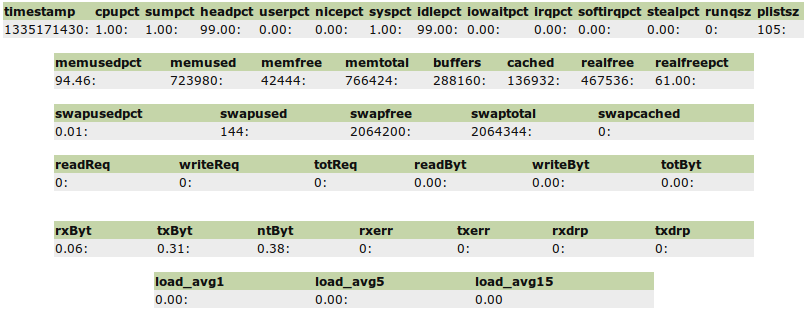
\includegraphics[scale=0.62]{sysrec_linux.png}
\caption{sysrec Linux}
\label{fig:sysrec.linux}
\end{figure}


\noindent
sysrec records system utilization along with certain other important metrics:
\begin{verbatim}
  CPU
   #01 timestamp  : seconds since Epoch
   #02 cpupct     : CPU Utilization, across all CPUs, percentage, gauge
   #03 sumpct     : sum of all CPUs Utilization, percentage, gauge
   #04 headpct    : headroom CPU available, all CPUs, percentage, gauge
   #05 userpct    : CPU Utilization User space in percent, gauge
   #06 nicepct    : CPU Utilization User space with nice priority, gauge
   #07 sysct      : CPU Utilization System space, gauge
   #08 idlepct    : CPU Utilization Idle state, gauge
   #09 iowaitcpt  : CPU Percentage in Idle state because an I/O, gauge
                    operation is waiting to complete, gauge
   #10 irqpct     : CPU Percentage servicing interrupts, gauge
   #11 softirqpct : CPU Percentage servicing softirqs, gauge
   #12 stealpct   : CPU Percentage of time spent in other operating systems
                    when running in a virtualized environment, gauge
   #13 runqsz     : run queue length, number of tasks waiting for run time
   #14 plistsz    : number of tasks in the task list

  MEM
   #15 memusedpct : size of used memory in percent, gauge
   #16 memused    : size of used memory in kilobytes, gauge (ext)
   #17 memfree    : size of free memory in kilobytes, gauge (ext)
   #18 memtotal   : size of memory in kilobytes, gauge (ext)
   #19 buffers    : size of buffers used from memory in kilobytes, gauge (ext)
   #20 cached     : size of cached memory in kilobytes, gauge (ext)
   #21 realfree   : size of memory is real free, gauge 
                     (memfree+buffers+cached) (ext)
   #22 realfreepct: size of memory is real free in percent of total memory,
                     gauge (ext)
   #23 swapusedpct: size of used swap space in percent, gauge
   #24 swapused   : size of swap space is used is kilobytes, gauge (ext)
   #25 swapfree   : size of swap space is free in kilobytes, gauge (ext)
   #26 swaptotal  : size of swap space in kilobytes, gauge (ext)
   #27 swapcached : memory that once was swapped out, is swapped back in 
                     but still also is in the swapfile, gauge (ext)

  DISK
   #28 readReq    : disk read requests, gauge
   #29 writeReq   : disk write requests, gauge
   #30 totReq     : disk read+write requests, gauge
   #31 readByt    : read bytes / sec, in KB, gauge
   #32 writeByt   : write bytes / sec, in KB, gauge
   #33 totByt     : read+write bytes / sec, in KB, gauge

  NET
   #34 rxByt      : received bytes /sec, in KB, gauge
   #35 txByt      : transmitted bytes /sec, in KB, gauge
   #36 ntByt      : received + transmitted bytes /sec, in KB, gauge
   #37 rxerr      : No. of errors that happend while received pckt/second
   #38 txerr      : No. of errors that happend while transmitting pckt/second
   #39 rxdrp      : No. of rx packets that were dropped per second
   #40 txdrp      : No. of tx packets that were dropped per second
 
   #41 avg_1      : LA of the last minute
   #42 avg_5      : LA of the last 5 minutes
   #43 avg_15     : LA of the last 15 minutes
\end{verbatim}


\subsubsection{Solaris}
sysrec on Solaris is a utility, part of K9Toolkit, author Brendan Gregg. 
The toolkit is a collection of free Perl scripts used to troubleshoot and 
observe Solaris systems. sysrec records 14 Solaris OS metrics on x64 and
sparcv9 platforms. The recorder has been modified to output its data as RRD.

\begin{figure}[!ht]
\centering
%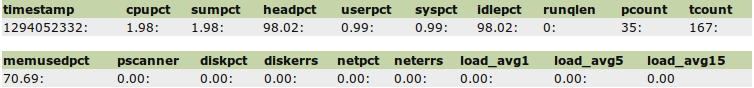
\includegraphics[width=145mm,height=15mm]{sysrec_sol.png}
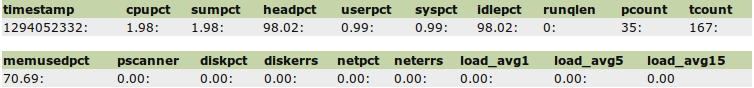
\includegraphics[scale=0.62]{sysrec_sol.png}
\caption{sysrec Solaris}
\label{fig:sysrec.linux}
\end{figure}

sysrec records system utilization and certain additional kernel statistics
used as a starting point in observing the system's general health. The output
from sysrec is displayed below:

\begin{verbatim}
  CPU
   #01 timestamp  : seconds since Epoch
   #02 cpupct     : CPU Utilization, across all CPUs, percentage, gauge
   #03 sumpct     : sum of all CPUs utilization, percentage, gauge
   #04 headpct    : headroom CPU available, all CPUs, percentage, gauge
   #05 userpct    : CPU Utilization User space, all cpus, percentage, gauge
   #06 syspct     : CPU Utilization System space, all cpus, percentage, gauge
   #07 idlepct    : CPU Utilization Idle state, all cpus, percentage, gauge
   #08 runqlen    : threads on the run queue, gauge
   #09 pcount     : current process count on the system
   #10 tcount     : current lwp count on the system

  MEM
   #11 memusedpct : size of used memory in percent, gauge
   #12 pscanner   : scan rate of the page scanner, gauge
 
  DISK
   #13 diskpct    : sum read+write across disks, percentage, gauge
   #14 diskerrs   : operations on the wait queue, gauge

  NET
   #15 netpct     : throughput, read+write bytes across NICs, percentage, gauge
   #16 neterrs    : number of errors due to buffer saturation

   #17 la_1       : Load Average 1min
   #18 la_5       : Load Average 5min
   #19 la_15      : Load Average 15min
\end{verbatim}


\noindent
\newline
Examples for Linux and Solaris operating systems:



\begin{center}
\begin{tabular}{lll}

\multicolumn{3}{c}{} \\
\textbf{Mode} & \textbf{Example} & \textbf{Description} \\ \hline
\newline

\multirow{4}{*}{\small{Default Mode}} & 
 \small{\emph{sysrec}} & \small{print summary since boot only}\\ & 
 \small{\emph{sysrec 60}} & \small{print every 60secs system stats}\\ & 
 \small{\emph{sysrec 1 5}} & \small{print 5 times, every 1secs system stats}\\ &
 \small{\emph{sysrec .5}} & \small{print every 0.5secs system stats}\\
 \hline

\multirow{2}{*}{\small{Extended Mode}} & 
 \small{} & \small{Linux Only} \\ &
 \small{\emph{sysrec -x 5}} & \small{print every 5secs extended 
    system stats, detailed memory figures}

\end{tabular}
\end{center}



% CPUREC
\subsection*{cpurec}
Records per CPU parameters from a Linux or Solaris system. On a multiprocessor
environment cpurec will display all CPUs and all parameters associated with them.

\subsubsection{Linux}
The recorder uses Sys::Statistics::Linux Perl module to extract and compute
all CPU statistics. cpurec records 10 Linux OS metrics on x64 and x86 platforms !
The recorder has been modified to output its data as RRD.  

\begin{figure}[!ht]
\centering
%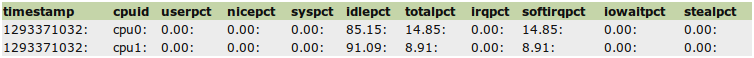
\includegraphics[width=145mm,height=12mm]{cpurec_lin.png}
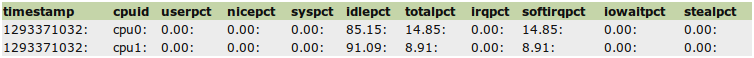
\includegraphics[scale=0.62]{cpurec_lin.png}
\caption{cpurec Linux}
\label{fig:cpurec_lin}
\end{figure}

\noindent
cpurec records system utilization along with certain other important metrics:

\begin{verbatim}
  #01 timestamp  : seconds since Epoch
  #02 cpuid      : CPU id
  #03 user       : CPU Utilisation User space percentage, gauge
  #04 nice       : CPU utilisation User space nice priority percentage, gauge
  #05 system     : CPU utilisation System space percentage, gauge
  #06 idle       : CPU Utilisation idle state percentage, gauge
  #07 total      : Total CPU Utilisation percentage, gauge
  #08 irq        : CPU Percentage servicing interrupts, gauge
  #09 softirq    : CPU Percentage servicing softirqs, gauge
  #10 iowait     : CPU Percentage in idle state because an I/O 
                    operation is waiting to complete, gauge
  #11 steal      : CPU Percentage of time spent in other operating systems 
                    when running in a virtualized environment, gauge
\end{verbatim}


\subsubsection{Solaris}
cpurec is a utility, collecting per-CPU data from kstat. The recorder outputs
its data under RRD format. cpurec records 12 Solaris OS metrics on x64 and
sparcv9 platforms !  cpurec used mainly to observe CPU activity and
analyse how the CPUs are used in the system. Useful for capacity planning.

\begin{figure}[!ht]
\centering
%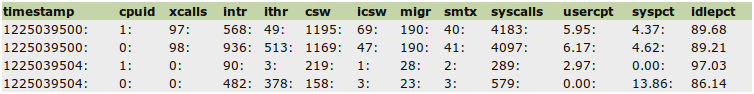
\includegraphics[width=145mm,height=18mm]{cpurec_sol.png}
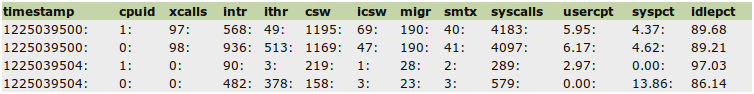
\includegraphics[scale=0.62]{cpurec_sol.png}
\caption{cpurec Solaris}
\label{fig:cpurec_sol}
\end{figure}

\noindent
Recording parameters:

\begin{verbatim}
  #01 timestamp: seconds since Epoch
  #02 Xcalls   : rate of multiprocessor cross calls, gauge
  #03 Intr     : rate of intrerrupts, gauge
  #04 iThr     : rate of interrupts threads, gauge
  #05 Csw      : rate of context switches, gauge
  #06 Icsw     : rate of involuntary context switches, gauge
  #07 Migr     : rate of migrations, gauge
  #08 Smtx     : rate of kernel mutexes, gauge
  #09 Syscalls : rate of system calls, gauge
  #10 User     : percentage of time spent in user mode, gauge
  #11 Sys      : percentage of time spent in sys mode, gauge
  #12 Idle     : percentage of time spent in idle mode, gauge
\end{verbatim}


\noindent
\newline
Examples for Linux and Solaris operating systems:


\begin{center}
\begin{tabular}{lll}
\multicolumn{3}{c}{} \\
\textbf{Mode} & \textbf{Example} & \textbf{Description} \\ \hline
\newline

\multirow{4}{*}{\small{Default Mode}} &
 \small{\emph{cpurec}} & \small{print summary since boot only}\\ &
 \small{\emph{cpurec 60}} & \small{print every 60secs per CPU stats}\\ &
 \small{\emph{cpurec 1 5}} & \small{print 5 times, every 1secs per CPU stats}\\ &
 \small{\emph{cpurec .5}} & \small{print every 0.5secs per CPU stats}\\
% \hline

%\multirow{1}{*}{\small{Extended Mode}} &
% \small{} & \small{} \\ &
% \small{\emph{sysrec -x 5}} & \small{print every 5secs extended
%    system stats, detailed memory figures}

\end{tabular}
\end{center}



%\subsection*{diskrec}
%Not yet available !



% NICREC
\subsection*{nicrec}
nicrec records per NIC statistics. Useful to measure the throughput of one
or many network cards or the number of errors during transmitting or receiving 
packets.

\subsubsection{Linux}
The recorder uses Sys::Statistics::Linux to fetch all metrics. nicrec records
19 Linux OS metrics on x64 and x86 platforms ! The recorder has been modified 
to output its data as RRD and no delta values are stored, but rather raw data.

\begin{figure}[!ht]
\centering
%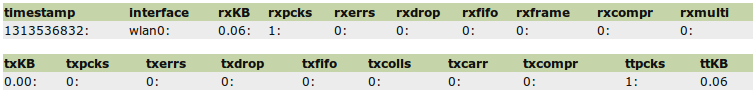
\includegraphics[width=145mm,height=18mm]{nicrec_lin.png}
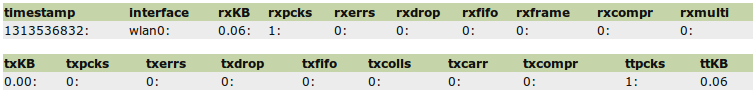
\includegraphics[scale=0.62]{nicrec_lin.png}
\caption{nicrec Linux}
\label{fig:nicrec_lin}
\end{figure}

\noindent
nicrec records per NIC metrics: 

\begin{verbatim}
  #01 timestamp  : seconds since Epoch
  #02 interface  : the interface name, NIC name
  #03 rxKB       : the no. of KBytes received/sec, gauge
  #04 rxpcks     : the no. of packets received/sec, gauge
  #05 rxerrs     : the no. of errors while received packets/sec, gauge
  #06 rxdrop     : the no. of packets that were dropped/sec, gauge
  #07 rxfifo     : the no. of FIFO overruns on received packets/sec, gauge
  #08 rxframe    : the no. of carrier errors on received packets/sec, gauge
  #09 rxcompr    : the no. of compressed packets received/sec, gauge
  #10 rxmulti    : the no. of multicast packets received/sec, gauge
  #11 txKB       : the no. of KBytes transmitted/sec, gauge
  #12 txpcks     : the no. of packets transmitted/sec, gauge
  #13 txerrs     : the no. of errors transmitting packets/sec, gauge
  #14 txdrop     : the no. of packets that were dropped/sec, gauge
  #15 txfifo     : the no. of FIFO overruns on transmitted packets/sec, gauge
  #16 txcolls    : the no. of collisions that were detected/sec, gauge
  #17 txcarr     : the no. of carrier errors on transmitted packets/sec, gauge
  #18 txcompr    : the no. of compressed packets transmitted/sec, gauge
  #19 ttpcks     : the no. of total packets (received + transmitted)/sec, gauge
  #20 ttKB       : the no. of total KBytes (received + transmitted)/sec, gauge
\end{verbatim}


\subsubsection{Solaris}
nicrec is a utility part of K9toolkit, author Brendan Gregg, printing network
traffic, KB/s transferred per network interface, packet counts and average
sizes. nicrec records 9 Solaris OS metrics on x64 and sparcv9 platforms ! 
The recorder outputs its data under RRD format.

\begin{figure}[!ht]
\centering
%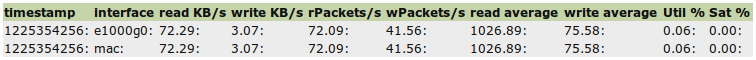
\includegraphics[width=145mm,height=12mm]{nicrec_sol.png}
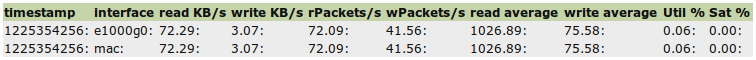
\includegraphics[scale=0.62]{nicrec_sol.png}
\caption{nicrec Solaris}
\label{fig:nicrec_sol}
\end{figure} 

\noindent
Recording parameters:
\begin{verbatim}
  #01 timestamp: seconds since Epoch
  #02 int      : interface
  #03 rKB/s    : read KB/s, gauge
  #04 wKB/s    : write KB/s, gauge
  #05 rPk/s    : read Packets/s, gauge
  #06 wPk/s    : write Packets/s, gauge
  #07 rAvs     : read Average size, bytes
  #08 wAvs     : write Average size, bytes
  #09 %Util    : utilisation (read+write)/nic speed, gauge
  #10 Sat      : Saturation: defer, nocanput, norecvbuf, noxmtbuf, gauge
\end{verbatim}

\noindent
\newline
Examples for Linux and Solaris operating systems:

\begin{center}
\begin{tabular}{lll}
\multicolumn{3}{c}{} \\
\textbf{Mode} & \textbf{Example} & \textbf{Description} \\ \hline
\newline

\multirow{4}{*}{\small{Default Mode}} &
 \small{\emph{nicrec}} & \small{print summary since boot only}\\ &
 \small{\emph{nicrec 60}} & \small{print every 60secs per NIC stats}\\ &
 \small{\emph{nicrec 1 5}} & \small{print 5 times, every 1secs per NIC stats}\\ &
 \small{\emph{nicrec .5}} & \small{print every 0.5secs per NIC stats}\\
% \hline

%\multirow{1}{*}{\small{Extended Mode}} &
% \small{} & \small{Linux Only} \\ &
% \small{\emph{sysrec -x 5}} & \small{print every 5secs extended
%    system stats, detailed memory figures}

\end{tabular}
\end{center}


\section{Specialized Recorders}
These are recorders specific for different applications or certain
parts of the operating system only. These are optional recorders and
should be enabled only on systems which require such monitoring.


% COREREC
\subsection*{corerec}
A SPARC processor specific recorder, responsible to report per core
utilization. This is a Solaris/SPARC system recorder only !

\subsubsection{Solaris}
corerec is a utility using corestat, from Cooltools, original project of
Sun Microsystems Inc. The output is not formatted for SDR Reporting module 
and it is simple as human readable format.

corerec is used to observe core utilization from a T1 or T2 processor. Since T1
and T2 have different registers for keeping track of the usage the corestat
utility has to be different for each case: corestat.t1 used for T1 processors
and corestat.t2 for T2. 

\noindent
Recording parameters:

\begin{verbatim}
%Usr: percentage user time
%Sys: percentage sys time
%Usr+Sys: both Usr + Sys
Avg: core utilization

The output from corerec is displayed below:

For a T2 processor:
Core,Int-pipe     %Usr     %Sys     %Usr+Sys 
    0,0           0.05      0.37      0.42 
    0,1           0.06      0.07      0.13 
    1,0           0.04      0.08      0.12 
    1,1           0.01      0.05      0.06 
    2,0           0.09      0.11      0.20 
    2,1           0.01      0.06      0.07 
    3,0           0.02      0.15      0.17 
    3,1           0.01      0.05      0.05 
    4,0           0.01      0.13      0.14 
    4,1           0.01      0.04      0.05 
    5,0           0.07      0.10      0.16 
    5,1           0.01      0.45      0.46 
    6,0           0.02      0.10      0.12 
    6,1           0.01      0.06      0.07 
    7,0           0.03      0.12      0.14 
    7,1           0.05      0.06      0.01 
-------------     -----     -----    ------ 
    Avg           0.03      0.12      0.15 

\end{verbatim}

Important to note here is that utilization for a T1 or T2 processor does not
simple mean data from vmstat, mpstat or sysrec, cpurecalone. You have to use 
corerec in order to gather the per core utilization figures. 



% JVMREC
\subsection*{jvmrec}
jvmrec records per JVM garbage collection statistics. It is very important to
understand and check how well your Java applications are running. For this we
will need to look and check internal Java Virtual Machine parameters, 
like the garbage collection statistics. The recorders uses jstat, part of 
standard JDK displaying its data under RRD format.


\subsubsection{Linux}
jvmrec records the GC statistics useful to understand how your JVMs are
running. jvmrec can easily filter certain JVMs using -f format option 
, where format is a Perl regexp. The format is used mainly to filter,
search over a number of running JVMs for a specific set and use only 
those ! jvmrec as well supports an extended mode, when used the utility 
will report Disk IO statistics along with GC activity. This is useful 
in cases a Java application is heavily GCing and it does create a lot of
Disk IO.

\noindent
Recording parameters:

\begin{verbatim}
  #01 timestamp  : seconds since Epoch
  #02 name.pid   : JVM name and process ID
  #03 S0         : Survivor S0 utilisation, percentage, gauge
  #04 S1         : Survivor S1 utilisation, percentage, gauge
  #05 Eden       : Eden space utilisation, percentage, gauge
  #06 Old        : Old space utilisation, percentage, gauge
  #07 Perm       : Permanent space utilisation, percentage, gauge
  #08 No.mGC     : Number of young generation GC events
  #09 Time.mGC   : Young generation garbage collection time, secs
  #10 No.MGC     : Number of full GC events
  #11 Time.MGC   : Full garbage collection time, secs
  #12 TotalGC    : Total garbage collection time, secs
  #13 utime      : The no. of jiffies scheduled in user mode
  #14 stime      : The no. of jiffies scheduled in kernel mode
  #15 size       : The total program size of the process
  #16 resident   : The resident set size, the text, data and stack space
  #17 nswap      : The size of swap space of the proces
  #18 syscr      : Number of read syscalls
  #19 rchar      : Bytes read from storage (might have been from pagecache)
  #20 read_bytes : Bytes really fetched from storage layer
  #21 syscw      : Numner of write syscalls
  #22 wchar      : Bytes written
  #23 write_bytes: Bytes sent to the storage layer
\end{verbatim}


\subsubsection{Solaris}
jvmrec records GC statistics useful to understand how your JVMs are
running. jvmrec is implemented as a KSH recorder on Solaris.

\noindent
Recording parameters:

\begin{verbatim}
  #01 timestamp : seconds since Epoch
  #02 zone.pid  : name of the zone and process ID
  #03 S0%       : Survivor S0 utilisation, percentage, gauge
  #04 S1%       : Survivor S1 utilisation, percentage, gauge
  #05 Eden%     : Eden space utilisation, percentage, gauge
  #06 Old%      : Old space utilisation, percentage, gauge
  #07 Perm%     : Permanent space utilisation, percentage, gauge
  #08 No.mGC    : Number of young generation GC events
  #09 Time.mGC  : Young generation garbage collection time, secs
  #10 No.MGC    : Number of full GC events
  #11 Time.MGC  : Full garbage collection time, secs
  #12 TotalGC   : Total garbage collection time, secs
\end{verbatim}

\noindent
\newline
Examples for Linux and Solaris operating systems:
\begin{center}
\begin{tabular}{lll}

\multicolumn{3}{c}{} \\
\textbf{Mode} & \textbf{Example} & \textbf{Description} \\ \hline
\newline

\multirow{2}{*}{\small{Default Mode}} & \small{\emph{jvmrec 60}} &
 \small{print every 60secs stats all JVMs}\\

 & \small{\emph{jvmrec 5 10}} & \small{print every 5secs JVM stats 10
samples}\\
 \hline

\multirow{3}{*}{\small{Filter Mode}} &
 \small{\emph{jvmrec -f weblogic 60}} &
 \small{print every 60secs Weblogic stats}\\

 & \small{\emph{jvmrec -f '-Dmyapp.Name' 60}} &
   \small{print every 60secs all Dmyapp.Name JVMs}\\

 & \small{\emph{jvmrec -f '\^{}(?!.*?esite).*' 60}} &
   \small{print every 60secs all JVMs which are not called esite}\\

\hline
\multirow{2}{*}{\small{Extended Mode}} &
 \small{} & \small{Linux Only} \\ &
 \small{\emph{jvmrec -xf 'com*' 360}} &
 \small{print every 360secs all com JVMs including extended statistics}\\

\end{tabular}
\end{center}




% NETREC
\subsection*{netrec}
netrec records per protocol statistics: TCP, UDP for example. It does use an 
extra operating system utility, netstat. The recorder outputs its data under 
RRD format.

\subsubsection{Linux}
netrec records per protocol statistics TCP, UDP from netstat utility. The 
recorder uses netstat binary, so this utulity should be present on your Linux
installation. The recorder has been modified to output its data as RRD and no
delta values are stored, but rather raw data.

\begin{figure}[!ht]
\centering
%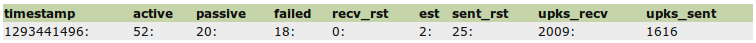
\includegraphics[width=145mm,height=9mm]{netrec_lin.png}
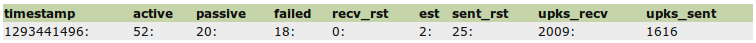
\includegraphics[scale=0.62]{netrec_lin.png}
\caption{netrec Linux}
\label{fig:netrec_lin}
\end{figure}

\noindent
Recording parameters:

\begin{verbatim}
  #01 timestamp  : seconds since Epoch
  #02 active     : TCP active connections, counter
  #03 passive    : TCP passive connections, counter
  #04 failed     : TCP failed connection attempts, counter
  #05 recv_rst   : TCP connection resets received, counter
  #06 est        : TCP connections established, gauge
  #07 sent_rst   : TCP resets sent, counter
  #08 upks_recv  : UDP packets received, counter
  #09 upks_sent  : UDP packets sent, counter
  #10 fast_retr  : Fast retransmits, counter
  #11 fwd_retr   : Forward retransmits, counter
  #12 slow_retr  : Retransmits in slow start, counter
\end{verbatim}




\subsubsection{Solaris}
netrec is a utility, reporting TCP, UDP and IP statistics from a running local
or global zone. If the system deploys one or more zones and if all zones share
same TCP/IP stack then you can simple use -s flag to report the numbers just
once. The recorder outputs its data under RRD format and no delta are stored !

\noindent
Recording parameters:

\begin{verbatim}
  #01 timestamp       : seconds since Epoch
  #02 zonename        : Solaris zone name
  #03 udpInDatagrams  : No. of UDP input datagrams
  #04 udpInErr        : No. of UDP input errors
  #05 udpOutDatagrams : No. of UDP output datagrams
  #06 udpOutErrors    : No. of UDP output errors
  #07 tcpActiveOpens  : No. of outgoing connections since boot, counter
  #08 tcpPassiveOpens : No. of incoming connections since boot, counter
  #09 tcpAttemptFails : No. of outgoing failures since boot, counter
  #10 tcpEstabResets  : No. of resets to terminate established connections
  #11 tcpCurrEstab    : No. of current established connections
  #12 tcpOutSegs      : Total no. of segments sent, counter
  #13 tcpOutDataSegs  : Sender total no. of data segments sent, counter
  #14 tcpOutDataBytes : Sender total no. of bytes in data segments sent,
                         counter
  #15 tcpRetransSegs  : Total no. of segments retransmitted
  #16 tcpRetransBytes : Sender total no. of bytes in segments retransmitted,
                         counter
  #17 tcpOutRsts      : No. of segments sent with RST flag, counter

  #18 tcpListenDrop   : Total no. of connections refused, backlog full
  #19 tcpListenDropQ0 : Total no. of connections refused, half-open queue full
  #20 tcpHalfOpenDrop : Total no. of connections dropped, full half-open queue
  #21 tcpOutSackRetrs : Total no. of retransmitted segments by SACK retrans
  #22 ipInHdrErr      : No. of dg discards for iph error
  #23 ipInAddrErr     : No. of dg discards for bad addr
  #24 ipInCksumErr    : No. of bad IP header checksum
  #25 tcpInErr        : Total no. of segments recv with error, counter
  #26 udpInCksumErr   : No. of UDP packets with bad UDP checksum, counter
\end{verbatim}



% PROCREC
\subsection*{procrec}
This is a Linux specific recorder. procrec records per process statistics: 
owner, state, nice, the priority of the process, the no. of light weight 
processes, the no. of open file descriptors, the no. of minor and major faults 
the process made and many other metrics. The recorder uses 
Sys::Statistics::Linux to fetch all metrics. The recorder has been modified to 
output its data as RRD and no delta values are stored, but rather raw data. 

\begin{figure}[!ht]
\centering
%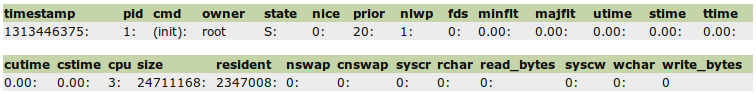
\includegraphics[width=145mm,height=20mm]{procrec_lin.png}
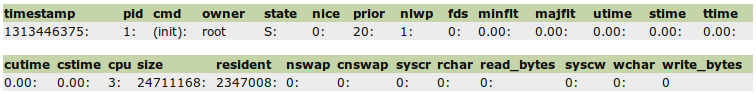
\includegraphics[scale=0.62]{procrec_lin.png}
\caption{procrec Linux}
\label{fig:procrec_lin}
\end{figure}

\noindent
Recording parameters:

\begin{verbatim}
  #01 timestamp  : seconds since Epoch
  #02 pid        : the process ID of the process
  #03 cmd        : command of the process
  #04 owner      : the owner of the process
  #05 state      : the status of the process
  #06 nice       : the nice level of the process
  #07 prior      : the priority of the process (+15)
  #08 nlwp       : the no. of light weight processes by this process
  #09 fds        : the no. of open file descriptors
  #10 minflt     : the no. of minor faults the process made
  #11 mayflt     : the no. of major faults the process made
  #12 utime      : the no. of jiffies proc have beed in user mode
  #13 stime      : the no. of jiffies proc have beed in kernel mode
  #14 ttime      : the no. of jiffies proc have beed (user + kernel)
  #15 cutime     : the no. of jiffies proc waited for childs in user mode
  #16 cstime     : the no. of jiffies proc waited for childs in kernel mode
  #17 cpu        : the CPU number the process was last executed on
  #18 size       : the total program size of the process, in bytes
  #19 resident   : the resident set size(the text, data, stack), in bytes
  #20 nswap      : the size of swap space of the process
  #21 cnswap     : the size of swap space of the childrens of the process
  #22 syscr      : number of read syscalls
  #23 rchar      : bytes read from storage (might have been from pagecache)
  #24 read_bytes : bytes really fetched from storage layer
  #25 syscw      : number of write syscalls
  #26 wchar      : bytes written
  #27 write_bytes: bytes sent to the storage layer
  #28 cmdline    : command line of the process (ext)
\end{verbatim}



% WEBREC
\subsection*{webrec}
This is a generic recorder, working under Linux or Solaris based
operating systems.  webrec is a utility based on Apache HTTPClient, 
written in Java intended to be used to measure response times for different 
HTTP actions: POST, GET. Currently webrec supports only GET HTTP methods. 
Work in under way to expand this to POST methods and authentication.

\begin{figure}[!ht]
\centering
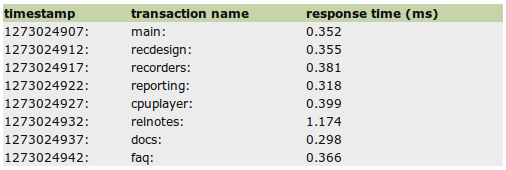
\includegraphics[width=105mm,height=35mm]{webrec.png}
\caption{webrec}
\label{fig:webrec}
\end{figure}

webrec checks for a master configuration file, called: webrec.conf located
under SDR/etc/ director, where SDR Recording module has been installed. It
parses the configuration file: webrec.conf and it retrieves the values for
timeout and the name definitions of each workload. For each workload it
creates a thread and its starting to follow each URL recording the response
times. WebRec supports Cookies as defined in RFC 2965 

webrec operates against one or many workloads. Workload defines a sequence of
URLs with the following properties:

\noindent
Recording parameters:

\begin{verbatim}
name    : name of the workload
delay   : delay after each URL (in seconds)
interval: the interval to invoke workloads (in seconds)
timeout : determines the timeout until a connection is
           etablished. A value of zero means the timeout is not used. The
           default value is zero. (in milliseconds)
\end{verbatim}



% ZONEREC
\subsection*{zonerec}
This is a Solaris only recorder, responsible to display per zone statistics. 
zonerec is a simple script calling prstat utility to report zone utilization in
human readable format. This data needs to be parsed and prepared in RRD
format. Future versions will include a new recorder which will output its data
to RRD format.

zonerec used to observe CPU and Mem utilization, as reported by prstat.



\begin{figure}[!ht]
\centering
%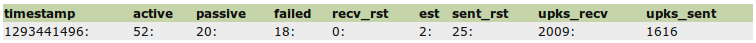
\includegraphics[width=145mm,height=9mm]{netrec_lin.png}
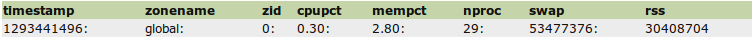
\includegraphics[scale=0.62]{zonerec_sol.png}
\caption{zonerec Solaris}
\label{fig:zonerec_sol}
\end{figure}

\noindent
Recording parameters:

\begin{verbatim}
  #01 timestamp: seconds since Epoch
  #02 zonename : Solaris zone name
  #03 zid      : Solaris zone id
  #04 cpu      : CPU utilisation, percentage, gauge
  #05 mem      : Mem utilisation, percentage, gauge
  #06 nproc    : no. of processes used by zoneid
  #07 swap     : total swap used by zoneid, includes tmpfs mounts, in bytes
  #08 rss      : resident set size, the amount of physical memory, in bytes
\end{verbatim}


% Transport Utilities
\section{Transport Utilities}
SDR Recording module contains some utilities to manage the recorded raw data: 
archive sdrd raw daily data, monitor and transport sdrd raw data changes 
to a reporting site for instant monitoring or transport archived data to a
reporting centralized site. For transport these tools use SSH2 or FTP protocols.

% RAW2DAY
\subsection*{raw2day}
raw2day is responsibile to create a compressed copy of the sdrd raw data, 
for the past day for archiving purposes. The utility, usually, operates in 
batch mode, at midnight, scheduled to run via crontab. By default the tool 
does not transport as well the data archived. To transport the archived data 
raw2day must be told to run the transport mode which supports SSH2 or FTP protocols.

\noindent
\newline
raw2day archives daily sdrd raw data and if neccesasrily transport it
to a dedicated reporting sserver:
\begin{verbatim}
USAGE: raw2day [-hV] [-t ftp|scp|sftp] [host...]
  e.g. raw2day               moves raw data to daily log
       raw2day -t ftp        switch transport to FTP
       raw2day -t sftp       switch transport to SFTP
       raw2day -t scp        switch transport to SCP
       raw2day -t sftp rep1  switch transport to SFTP and 
                              transport data to rep1 reporting server
NOTES:
   sdr.conf  : raw2day uses sdr.conf XML configuration file !
\end{verbatim}


\noindent
\newline
Examples for Linux and Solaris operating systems:

\begin{center}
\begin{tabular}{lll}

\multicolumn{3}{c}{} \\
\textbf{Mode} & \textbf{Example} & \textbf{Description} \\ \hline
\newline

\multirow{1}{*}{\small{Default Mode}} & 
 \small{\emph{raw2day}} & \small{archives daily sdrd raw data}\\
 \hline

\multirow{3}{*}{\small{Transport Mode}} & 
 \small{\emph{raw2day -t ftp}} & \small{archives daily sdrd raw data and transports it using FTP}\\ & 
 \small{\emph{raw2day -t sftp}} & \small{archives daily sdrd raw data and transports it using SFTP}\\ &
 \small{\emph{raw2day -t sftp rep1}} & \small{switch transport to SFTP and transport data to rep1 reporting server}
\end{tabular}
\end{center}

% RAW2DAY
\subsection*{sender}
sender  is  responsible  for sending sdrd raw data updates to a backend
reporting system for instant monitoring:  updates,  plotting.  It  uses
SSH2 for a secure transport between each recording host and the backend
reporting server.

During its start, sender, will look  for  the  main  SDR  configuration
file,  sdr.conf  to  fetch what sdrd raw data files will look after and
where to transport the changes. Make sure you  have  a  single  backend
reporting  server defined currently under sdr.conf ! Currently the last
definition of the reporting host will be used.

The utility uses SSH2 transport libraries to create a  connection  from
each  recording host to a backend reporting system and send all updates
via this connection. In case  of  a  temporarily  failure  sender  will
reopen the SSH2 connections and start sending the updates again. If for
some reasons the backend system wont answer in a  proper  time,  sender
will wait until the reporting will allow connections or comeback alive.
In case of a fatal connection failure sender will wait permanentely for
the backend reporting server.

By  default,  sender will output all its messages and errors under pre‐
fix/log/sender.log log file. For example the default installation will
have sender output all info and error messages under /opt/sdr/log/sender.log

\noindent
\newline
\begin{verbatim}
USAGE: sender [-t secs] [-hV] | [interval]
OPTIONS:
  -t        : timeout in seconds
  -h        : help information
  -V        : release version
  interval  : maximum number of seconds between samples, default 60, will 
              never spend more than that without checking data

 e.g. sender     check and send sdrd raw data, every 60 secs
      sender 10  check and send sdrd raw data, every 10 secs

NOTES:
 sdr.conf: sender uses sdr.conf XML configuration file ! Make sure you
 have a functional sdr.conf installed or define where sdr.conf
 is found using SDR_ROOT variable
\end{verbatim}



\endinput
